% Claim:
%   Related work is organized as a conceptual boundary map by runtime question,
%   not a product comparison. Each citation supports a specific distinction
%   between adjacent systems and OpenRath's session-centered runtime value.
% Evidence:
%   Primary sources for reasoning/tool agents, multi-agent frameworks,
%   runtime/observability layers, memory and retrieval, evaluation environments,
%   and provenance standards. External links checked May 29, 2026.
% Open questions:
%   Pin exact source versions and access dates in the release source snapshot.

The agent ecosystem is converging on a specialized runtime stack: reasoning-and-acting
methods, multi-agent frameworks, durable graph runtimes, tracing SDKs, tool/data
protocols, real-environment benchmarks, and provenance standards each own one
layer. The open design question is the \emph{crossing object}---what state can
move through these layers while keeping conversation, lineage, placement, tool
effects, memory, and artifacts together. We survey these areas by that question
and, for each, mark the distinction from OpenRath's \texttt{Session}.

\subsection{Tool-Using and Acting Agents}

Chain-of-thought prompting and self-consistency elicit and stabilize
intermediate reasoning at inference time~\cite{cot,selfconsistency}. ReAct
interleaves reasoning with environment-directed actions~\cite{react}, and MRKL
combines a model with external knowledge and discrete reasoning
modules~\cite{mrkl}. Tool use itself is taught or routed by
Toolformer~\cite{toolformer}, HuggingGPT's controller over expert
models~\cite{hugginggpt}, and Gorilla's retrieval-grounded API
calls~\cite{gorilla}, and is studied at scale by ToolLLM, API-Bank, and
ToolAlpaca~\cite{toolllm,apibank,toolalpaca}; Tree of Thoughts adds deliberate
search with backtracking~\cite{tot}, an inference-time search rather than a
persistent, replayable branch. These works advance \emph{how} a model reasons
and acts; OpenRath is complementary, making the runtime state those actions
produce---lineage, tool evidence, placement---a first-class value.

\subsection{Multi-Agent Frameworks}

AutoGen frames applications as multi-agent conversations~\cite{autogen}, CAMEL
studies role-playing communicative agents~\cite{camel}, MetaGPT encodes
standardized operating procedures into a collaboration pipeline~\cite{metagpt},
ChatDev runs a virtual software company over a chat chain~\cite{chatdev}, and
AgentVerse studies dynamic group collaboration and emergent
behavior~\cite{agentverse}. These contribute orchestration patterns. The
distinction is one of object boundary: where MetaGPT's SOP governs \emph{which
role acts when}, OpenRath governs \emph{what value the roles pass}, so
multi-agent composition needs no second, framework-private state object.

\subsection{Runtime State, Protocols, and Observability}

LangGraph exposes checkpointed graph state with history and time travel to
replay or fork from a checkpoint~\cite{langgraph-persistence,langgraph-timetravel};
an OpenRath \texttt{Session}, by contrast, is the value the program itself passes
and forks, not a scheduler checkpoint. The OpenAI Agents SDK records traces and
spans over generations, tool calls, handoffs, and guardrails and composes agents
from those parts~\cite{openai-agents-tracing,openai-agents-docs}, and
OpenTelemetry treats spans as an observer-facing signal~\cite{opentelemetry};
traces describe \emph{what was observed} after the fact, whereas \texttt{Session}
is written for the program, so its evidence is the value itself. Connectivity is
standardized by the Model Context Protocol~\cite{mcp-docs,anthropic-mcp} and
interface descriptions such as OpenAPI~\cite{openapi}. The dataflow-runtime
analogy is instructive: TensorFlow represents computation and shared state as a
graph~\cite{tensorflow}, while OpenRath keeps the value imperative and lets
lineage, placement, and evidence travel with it.
Table~\ref{tab:related-runtime-landscape} summarizes the object-boundary
question each layer leaves open.

\begin{figure}[!htbp]
\centering
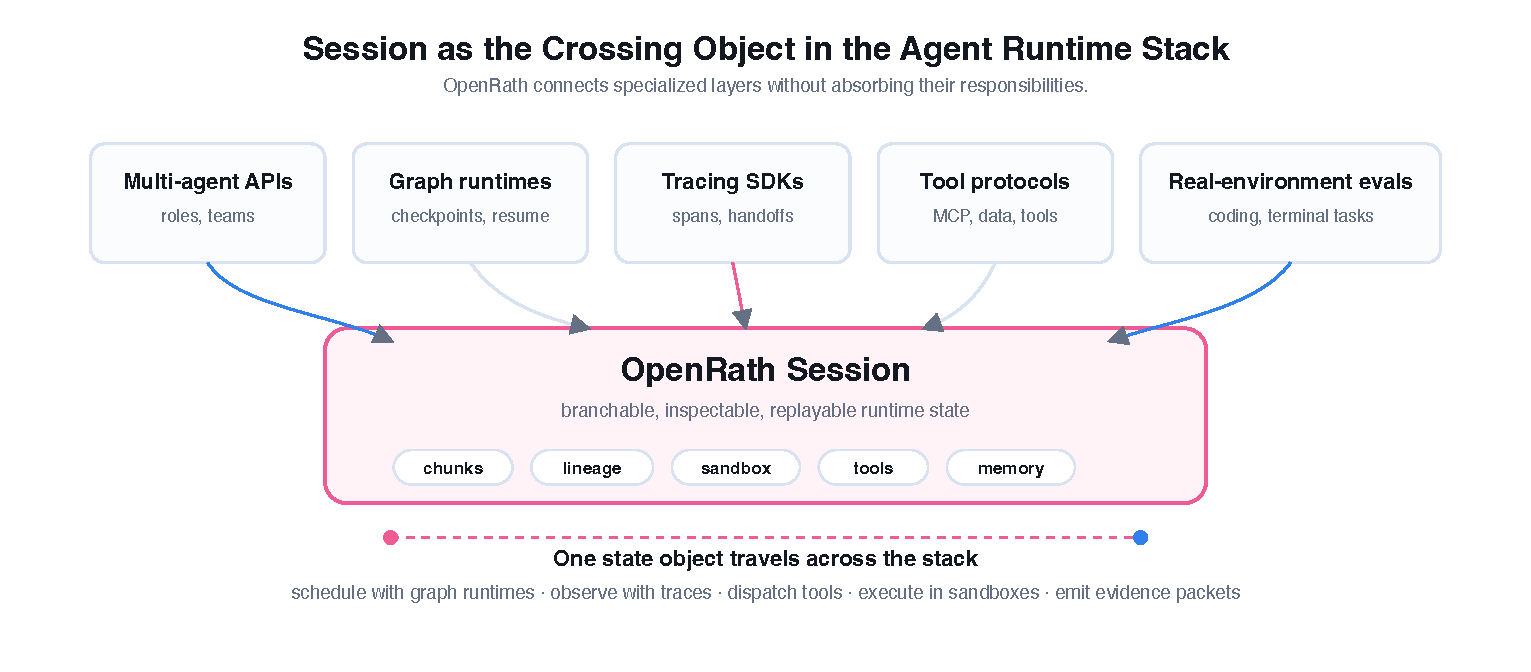
\includegraphics[width=0.96\linewidth]{assets/fig-runtime-stack-positioning.pdf}
\caption{OpenRath's ecosystem role is a crossing-object boundary. It can work
with specialized agent APIs, graph runtimes, tracing SDKs, tool protocols,
sandbox providers, and evaluation harnesses by making their effects visible in
one \texttt{Session}.}
\label{fig:runtime-stack-positioning}
\end{figure}

\begin{table}[H]
\vspace{0.2em}
\centering
\caption{Runtime-stack trends and OpenRath's intended boundary.}
\label{tab:related-runtime-landscape}
\begin{tabularx}{\linewidth}{@{}>{\raggedright\arraybackslash}p{0.23\linewidth}>{\raggedright\arraybackslash}X>{\raggedright\arraybackslash}X@{}}
\toprule
Trend & What became first-class & Remaining object-boundary question \\
\midrule
Multi-agent APIs & Agent roles, teams, group chats, and workflow patterns. & What state moves between roles besides transcript text? \\
Durable graph runtimes & Checkpoints, thread state, state history, resume, and time travel. & What session-level evidence should a graph node carry? \\
Tracing SDKs & Model spans, tool calls, handoffs, guardrails, and custom events. & What runtime value should traces attach to and replay from? \\
Tool/data protocols & Standardized access to external tools, data, and workflows. & How do external effects return as lineage, artifacts, and backend evidence? \\
Real-environment benchmarks & Repository tasks, terminal tasks, GUI/CLI environments, tests, and scored outcomes. & Can reviewers inspect how the outcome was produced? \\
\bottomrule
\end{tabularx}
\vspace{0.2em}
\end{table}

\subsection{Memory and Retrieval}

A large body of work studies what an agent should remember and how it should
retrieve it. At the agent level, Reflexion converts feedback from failed
attempts into natural-language reflections held in an episodic buffer, so later
attempts improve~\cite{reflexion}; Generative Agents maintain a long-running
memory stream that is retrieved, reflected upon, and compiled into
plans~\cite{generative-agents}; and MemGPT adopts the operating-system idea of a
memory hierarchy, paging information between a bounded context window and
external storage to sustain long interactions~\cite{memgpt}. Voyager carries
this toward lifelong skill acquisition, growing a reusable library of verified
behaviors from environment feedback~\cite{voyager}. OpenRath does not propose a new memory model; it simply makes memory operations session-visible, so recall and commit are recorded as explicit runtime events on \texttt{Session} rather than hidden inside the prompt.


\subsection{Agent Benchmarks and Environments}

Interactive evaluation spans AgentBench~\cite{agentbench} and $\tau$-bench's
tool-agent-user setting with database-state checks~\cite{taubench}; software
engineering through SWE-bench~\cite{swebench}, SWE-agent's agent-computer
interface~\cite{swe-agent}, and the human-filtered SWE-bench Verified
subset~\cite{swebench-verified}; terminals through Terminal-Bench, TerminalWorld,
and task-alignment studies~\cite{terminal-bench,terminalworld,tab-benchmark}; and
web, desktop, and embodied settings including WebArena, VisualWebArena,
WorkArena, OSWorld, WebShop, Mind2Web, ALFWorld, ScienceWorld, GAIA, and
TheAgentCompany~\cite{webarena,visualwebarena,workarena,osworld,webshop,mind2web,alfworld,scienceworld,gaia,theagentcompany}.
These score outcomes inside realistic environments; OpenRath's complementary
question is whether the trajectory that produced an outcome is inspectable and
replayable---a precondition for trustworthy scoring.

